\documentclass[11pt, a4paper]{article}
\usepackage[utf8]{inputenc}
\usepackage[T1]{fontenc}
\usepackage[english]{babel}
\usepackage{geometry}
\usepackage{booktabs}
\usepackage{graphicx}
\usepackage{hyperref}
\usepackage{float}
\usepackage{xcolor}
\usepackage{caption}
\usepackage{tikz}
\usepackage{pgfplots}
\pgfplotsset{compat=1.18}

% Page geometry
\geometry{left=2.5cm, right=2.5cm, top=2.5cm, bottom=2.5cm}

% Custom commands - product name and company
\newcommand{\modelname}{Operator}
\newcommand{\company}{Agible}
\newcommand{\claude}{Claude 4.5 Opus}

% Chart style matching the reference photo (log scale, step functions)
\pgfplotsset{
    inferencechart/.style={
        width=15cm,
        height=9cm,
        xlabel={Max Steps Allowed},
        ylabel={Normalized Score},
        xmin=0, xmax=1000,
        ymin=-5, ymax=105,
        xmode=log,
        log basis x={10},
        xtick={1,10,100,1000},
        xticklabels={{$1$}, {$10^1$}, {$10^2$}, {$10^3$}},
        ytick={0,20,40,60,80,100},
        grid=major,
        major grid style={line width=.1pt, draw=gray!30},
        axis lines=left,
        line width=1.2pt,
        tick style={line width=0.8pt, black},
        label style={font=\small},
        title style={font=\bfseries\boldmath, align=center},
        legend style={
            at={(0.02,0.98)}, 
            anchor=north west, 
            draw=none, 
            fill=white,
            font=\small,
            row sep=2pt
        }
    }
}

\title{\textbf{Introducing \modelname} \\ \large A Powerful Multimodal Agent for Autonomous Computer Control}
\author{The \company{} Team}
\date{\today}

\begin{document}

\maketitle

\begin{abstract}
Today we introduce \modelname{} — a powerful multimodal agent built on a state-of-the-art vision-language model. It is capable of effectively performing diverse tasks in virtual worlds. Using a novel foundational architecture, \modelname{} integrates advanced reasoning enabled by reinforcement learning. This allows the model to reason before taking action, significantly enhancing its performance and adaptability, particularly in inference-time scaling. Our model achieves state-of-the-art results on various standard benchmarks, demonstrating strong reasoning capabilities and notable improvements over previous systems.
\end{abstract}

\section{Introduction}
\modelname{} represents a breakthrough in our efforts to enhance foundation model reasoning through gameplay and complex tool use. Compared to domains like mathematics or coding, interacting with user interfaces relies more on intuitive thinking and common sense, as well as precise visual grounding — making it an ideal domain for evaluating and improving general reasoning abilities.

\section{Comprehensive Computer Use}
\modelname{} establishes new state-of-the-art benchmark results. Its superiority is consistently demonstrated across multiple benchmarks spanning computer use, browser use, and phone use.

\begin{table}[H]
    \centering
    \caption{Performance on Computer Use Benchmarks}
    \label{tab:computer_use}
    \resizebox{\textwidth}{!}{%
    \begin{tabular}{llcccc}
        \toprule
        \textbf{Task Type} & \textbf{Benchmark} & \textbf{\modelname} & \textbf{OpenAI CUA} & \textbf{\claude} & \textbf{Previous SOTA} \\
        \midrule
        Computer Use & OSworld (100 steps) & 42.5 & 36.4 & 28.0 & 38.1 (200 steps) \\
                     & Windows Agent Arena (50 steps) & 42.1 & --- & --- & 29.8 \\
        \midrule
        Browser Use & WebVoyager & 84.8 & 87.0 & 84.1 & 87.0 \\
                    & Online-Mind2web & 75.8 & 71.0 & 62.9 & 71.0 \\
        \midrule
        Phone Use & Android World & 64.2 & --- & --- & 59.5 \\
        \bottomrule
    \end{tabular}%
    }
\end{table}

\section{GUI Grounding}
The high agentic performance of \modelname{} is grounded in its ability to accurately locate elements on screen. \modelname{} demonstrates significant improvement over previous SOTA in GUI Grounding tasks, particularly on the challenging ScreenSpotPro benchmark.

\begin{table}[H]
    \centering
    \caption{GUI Grounding Performance}
    \begin{tabular}{lcccc}
        \toprule
        \textbf{Benchmark} & \textbf{\modelname} & \textbf{OpenAI CUA} & \textbf{\claude} & \textbf{Previous SOTA} \\
        \midrule
        ScreenSpot-V2 & 94.2 & 87.9 & 87.6 & 91.6 \\
        ScreenSpotPro & 61.6 & 23.4 & 27.7 & 43.6 \\
        \bottomrule
    \end{tabular}
\end{table}

\section{Inference Time Scaling}
The following chart demonstrates the characteristic relationship between performance and allowed step count (inference-time scaling), typical for gaming and agentic tasks.

\begin{figure}[H]
    \centering
    \begin{tikzpicture}
        \begin{axis}[
            inferencechart,
            title={GAME INFERENCE TIME SCALING},
        ]
            % Blue line - Operator (steep growth)
            \addplot[color=blue!80!black, const plot mark mid, line width=1.4pt] coordinates {
                (5, 0) (10, 8) (20, 15) (30, 22) (50, 30) (70, 38) 
                (100, 48) (150, 58) (200, 63) (300, 70) (400, 73) 
                (500, 78) (600, 82) (700, 87) (800, 90) (900, 96) (1000, 100)
            };
            
            % Orange line - Claude (moderate growth)
            \addplot[color=orange!90!black, const plot mark mid, line width=1.4pt] coordinates {
                (5, 0) (10, 2) (20, 5) (30, 8) (50, 12) (70, 16) 
                (100, 20) (150, 24) (200, 26) (300, 27) (400, 28) 
                (500, 29) (600, 30) (700, 31) (800, 31.5) (900, 32) (1000, 32)
            };
            
            % Purple line - OpenAI CUA (slow growth/plateau)
            \addplot[color=violet!80!black, const plot mark mid, line width=1.4pt] coordinates {
                (5, 0) (10, 1.5) (20, 3) (30, 4.5) (50, 6) (70, 7) 
                (100, 8.5) (150, 9.5) (200, 10.5) (300, 11) (400, 11) 
                (500, 11) (600, 11) (700, 11) (800, 11) (900, 11) (1000, 11)
            };
            
            \legend{\modelname, \claude, OpenAI CUA}
        \end{axis}
    \end{tikzpicture}
    \caption{Normalized score as a function of maximum allowed steps for different models}
\end{figure}

\section{Execution Trace Example}
Below is an abbreviated execution trace demonstrating \modelname{}'s ability to handle complex cross-application tasks (LibreOffice Calc $\to$ Writer) with self-correction.

\begin{quote}
    \textbf{User Query:} Can you help transfer data from LibreOffice Calc to a LibreOffice Writer table while preserving the original formatting? Save the document as "price.docx" on the desktop.
\end{quote}

\noindent\textbf{Trace Summary:}
\begin{enumerate}
    \item \textbf{Selection:} The agent attempts to select A1:E15. Self-corrects (steps 1--5) upon detecting incomplete selection, succeeds at step 6.
    \item \textbf{Navigation:} Copies data (Ctrl+C), opens Writer, navigates to Table menu.
    \item \textbf{Correction:} Realizes that a $2\times2$ table is insufficient. Reasons: \textit{"The data spans A1:E15, meaning I need a 15$\times$5 table."}
    \item \textbf{Configuration:} Sets columns=5, rows=15 (steps 12--16).
    \item \textbf{Finalization:} Pastes data, saves file, performs visual verification.
\end{enumerate}

\begin{figure}[H]
    \centering
    \fbox{\parbox{0.9\textwidth}{
        \centering
        \vspace{0.5cm}
        \href{https://github.com/agible-ai/operator/blob/main/IMG_0043.gif}{\Large \textsf{[Video Demonstration of Task Execution]}}\\[0.3cm]
        \texttt{https://github.com/agible-ai/operator/blob/main/IMG\_0043.gif}\\[0.3cm]
        \small Demonstration of cross-application data migration (Calc $\rightarrow$ Writer)\\
        \small with formatting preservation and file saving
        \vspace{0.5cm}
    }}
    \caption{Video example of task execution (click to view GIF)}
    \label{fig:demo}
\end{figure}

\section{Versatility and Generalization}
Although \modelname{} was not specifically trained for "deep research" tasks, we demonstrate its generalization capabilities on challenging web benchmarks.

\begin{table}[H]
    \centering
    \caption{Web Browsing Generalization}
    \begin{tabular}{lccc}
        \toprule
        \textbf{Benchmark} & \textbf{\modelname{} w/ GUI} & \textbf{GPT-4.5} & \textbf{GPT-4o w/ search API} \\
        \midrule
        SimpleQA & 83.8 & 60.0 & 90.0 \\
        BrowseComp & 2.3 & 0.6 & 1.9 \\
        \bottomrule
    \end{tabular}
\end{table}

\section{Gameplay Capabilities}
Games represent a critical frontier for multimodal agents. We tested 14 games from poki.com (up to 1,000 steps per game). Results are normalized relative to the maximum score (100).

\begin{figure}[H]
    \centering
    \begin{tikzpicture}
        \begin{axis}[
            inferencechart,
            title={LEARNING DYNAMICS IN GAMEPLAY TASKS},
            xlabel={Interaction Step Count},
            legend style={at={(0.02,0.98)},anchor=north west, fill=white, fill opacity=0.9, text opacity=1},
        ]
            % Operator - converges to 100%
            \addplot[color=blue!70!black, smooth, tension=0.15, line width=1.3pt] coordinates {
                (5, 2) (10, 10) (20, 22) (50, 45) (100, 68) (200, 85) 
                (400, 94) (600, 98) (800, 99.5) (1000, 100)
            };
            
            % Claude - moderate result
            \addplot[color=orange!80!red, smooth, tension=0.15, line width=1.3pt] coordinates {
                (5, 0) (10, 3) (20, 8) (50, 15) (100, 22) (200, 28) 
                (400, 31) (600, 32) (800, 32) (1000, 32)
            };
            
            % OpenAI CUA - below average
            \addplot[color=violet!70!black, smooth, tension=0.15, line width=1.3pt] coordinates {
                (5, 1) (10, 4) (20, 9) (50, 16) (100, 20) (200, 23) 
                (400, 24) (600, 24) (800, 24) (1000, 24)
            };
            
            % 100% line
            \addplot[color=gray, dashed, line width=1pt, domain=5:1000] {100};
            
            \legend{\modelname, \claude, OpenAI CUA, Reference Maximum}
        \end{axis}
    \end{tikzpicture}
    \caption{Comparative learning dynamics: experience accumulation in gaming environments}
\end{figure}

\begin{table}[H]
    \centering
    \caption{Gameplay Performance (Normalized)}
    \label{tab:gameplay}
    \resizebox{\textwidth}{!}{%
    \begin{tabular}{lccc}
        \toprule
        \textbf{Game} & \textbf{OpenAI CUA} & \textbf{\claude} & \textbf{\modelname} \\
        \midrule
        2048 & 31.04 & 43.05 & \textbf{100.00} \\
        cubinko & 0.00 & 0.00 & \textbf{0.00} \\
        energy & 32.80 & 41.60 & \textbf{100.00} \\
        free-the-key & 0.00 & 0.00 & \textbf{100.00} \\
        Gem-11 & 46.27 & 0.00 & \textbf{100.00} \\
        hex-frvr & 92.25 & 30.76 & \textbf{100.00} \\
        Infinity-Loop & 23.08 & 2.31 & \textbf{100.00} \\
        Maze: Path of Light & 35.00 & 82.00 & \textbf{100.00} \\
        shapes & 52.18 & 6.26 & \textbf{100.00} \\
        snake-solver & 42.86 & 42.86 & \textbf{100.00} \\
        wood-blocks-3d & 2.02 & 0.00 & \textbf{100.00} \\
        yarn-untangle & 44.56 & 13.77 & \textbf{100.00} \\
        laser-maze-puzzle & 80.00 & 28.00 & \textbf{100.00} \\
        tiles-master & 78.27 & 52.18 & \textbf{100.00} \\
        \bottomrule
    \end{tabular}%
    }
\end{table}

\section{Additional Scaling Metrics}

\begin{figure}[H]
    \centering
    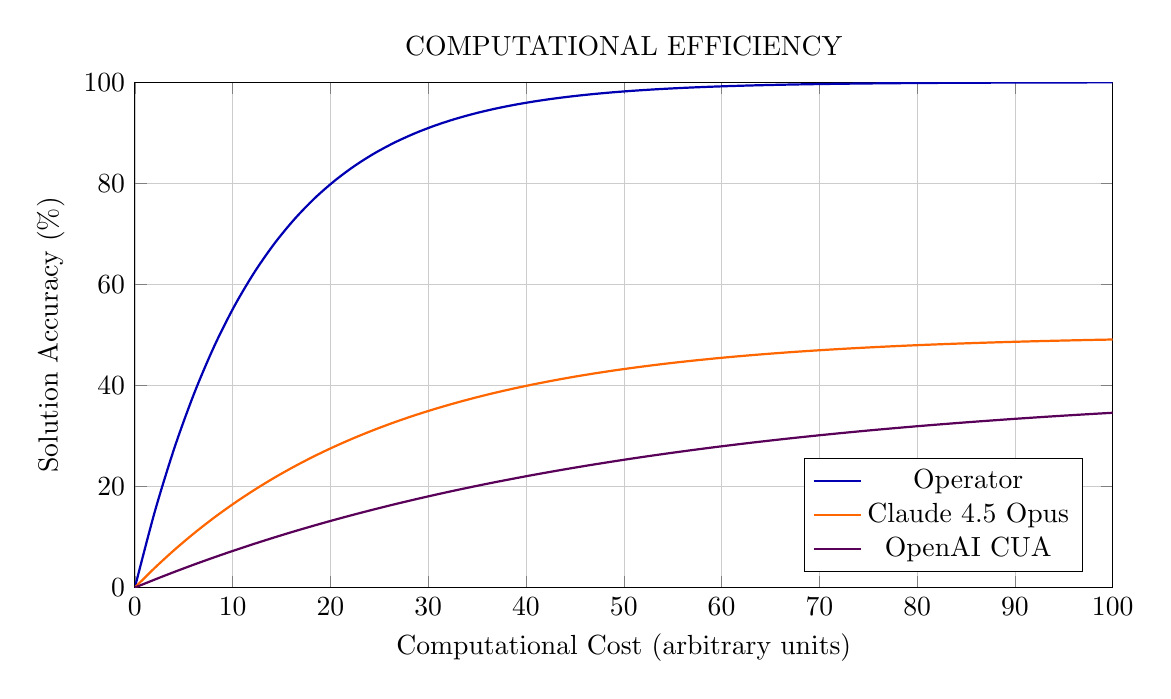
\begin{tikzpicture}
        \begin{axis}[
            width=14cm,
            height=8cm,
            xlabel={Computational Cost (arbitrary units)},
            ylabel={Solution Accuracy (\%)},
            xmin=0, xmax=100,
            ymin=0, ymax=100,
            grid=both,
            major grid style={line width=.2pt, draw=gray!40},
            title={COMPUTATIONAL EFFICIENCY},
            legend pos=south east,
        ]
            % Operator curve (fast saturation)
            \addplot[color=blue!70!black, thick, smooth, domain=0:100, samples=50] {100*(1-exp(-0.08*x))};
            
            % Claude curve
            \addplot[color=orange!80!red, thick, smooth, domain=0:100, samples=50] {50*(1-exp(-0.04*x))};
            
            % OpenAI curve
            \addplot[color=violet!70!black, thick, smooth, domain=0:100, samples=50] {40*(1-exp(-0.02*x))};
            
            \legend{\modelname, \claude, OpenAI CUA}
        \end{axis}
    \end{tikzpicture}
    \caption{Accuracy as a function of computational cost}
\end{figure}

\section{Limitations}
Despite the progress, \modelname{} has limitations:
\begin{enumerate}
    \item \textbf{Safety:} High GUI performance may lead to misuse (bypassing CAPTCHA). Internal safety evaluations are ongoing.
    \item \textbf{Computational Resources:} The model requires significant resources for extended scenarios.
    \item \textbf{Perception Errors:} Hallucinations and incorrect GUI element identification may occur in unfamiliar environments.
\end{enumerate}

\end{document}